\begin{tikzpicture}
	\def\w{2}
	\begin{scope}
		\begin{axis}
		[
			domain=0:2,
			samples=100,
			axis lines=center,
	    		xtick=\empty,
	    		ytick=\empty,	
			ymin=-1.2,   
			ymax=1.2,
			xmin=0,
			xmax=20,
			x=8cm,
		]
		\addplot [mark=none, ultra thick, blue, smooth] {cos(\w*deg(2*pi*x))};
		\addplot [ycomb, mark=none, samples=96,  thick, red] {cos(\w*deg(2*pi*x))};
		\end{axis}
	\end{scope}
	
	\def\wa{16}
	\begin{scope}[yshift=-8cm]
		\begin{axis}
		[
			domain=0:3*pi,
			samples=100,
			axis lines=center,
	    		xtick=\empty,
	    		ytick=\empty,	
			ymin=-1.2,   
			ymax=1.2,
			xmin=0,
			xmax=20,
			x=2cm,
		]
		\addplot [mark=none, ultra thick, blue, smooth] {cos(\wa*deg(x))};
		\addplot [ycomb, samples=36, mark=none, ultra thick, red] {cos(\w*deg(x))};
		\end{axis}
	\end{scope}	


\end{tikzpicture}